\documentclass[11pt,a4paper,11pt]{report}


\usepackage{geometry}
\usepackage{graphicx}
\geometry{hmargin=2.5cm,vmargin=2.0cm}
\usepackage[french]{babel}
\usepackage[T1]{fontenc}
\usepackage[utf8]{inputenc}
\usepackage{titlesec}
\usepackage{fancyhdr}
\usepackage{wrapfig}
\usepackage{SIunits}
\usepackage{amsmath}
\usepackage[final]{pdfpages}
\usepackage{bm}
\usepackage{array}
\usepackage{tabularx}
\usepackage[hyphens]{url} %pour retour à la ligne pour les liens
	\def\UrlBreaks{\do\.\do\@\do\\\do\/\do\!\do\_\do\|\do\;\do\>%
\do\]\do\)\do\,\do\?\do\'\do+\do\=\do\#\do\a\do\b\do\c\do\d\do\e\do\f\do\g\do\h\do\i\do\j\do\k\do\l\do\m\do\n\do\o\do\p\do\q\do\r\do\s\do\t\do\u\do\v\do\w\do\x\do\y\do\z%
\do\A\do\B\do\C\do\D\do\E\do\F\do\G\do\H\do\I\do\J\do\K\do\L\do\M\do\N\do\O\do\P\do\Q\do\R\do\S\do\T\do\U\do\V\do\W\do\X\do\Y\do\Z%
\do\1\do\2\do\3\do\4\do\5\do\6\do\7\do\8\do\9\do\%\do\=}%
\usepackage{lscape}
\usepackage{footnote}
\pagestyle{fancy}
\titleformat{\chapter}[hang]{\bf\huge}{\thechapter}{2pc}{}

\setcounter{secnumdepth}{3}
\setcounter{tocdepth}{3}


% FONCTIONS CREES POUR LES TABLES DE FIGURES ET LISTE DE TABLEAU

\let\pagebreakORIG\pagebreak
\let\clearpageORIG\clearpage
\let\cleardoublepageORIG\cleardoublepage
 
\ifx \removepagebreak \undefined
	\newcommand{\removepagebreak}{\renewcommand{\pagebreak}{}\renewcommand{\clearpage}{}\renewcommand{\cleardoublepage}{}}
\fi
 
\ifx \restorepagebreak \undefined
	\newcommand{\restorepagebreak}{\renewcommand{\pagebreak}{\pagebreakORIG}\renewcommand{\clearpage}{\clearpageORIG}\renewcommand{\cleardoublepage}{\cleardoublepageORIG}}
\fi

%%%%%%%%%%%%%%%%%%%%%%%%%%%%%%%%%%%%%%%%%%%%%%%%%%%%%%%%%%%%%%%%%%%%%%%%

\titlespacing{\chapter}{0pt}{*3}{*5}


\begin{document}

\fancyhead[L]{Rapport intermédiaire}
\fancyhead[R]{\og Le Thermostat Intelligent \fg}
\renewcommand\thesection{\arabic{section}}

\begin{titlepage}

\newcommand{\HRule}{\rule{\linewidth}{0.6mm}} % Defines a new command for the horizontal lines, change thickness here

\center % Center everything on the page
 
%----------------------------------------------------------------------------------------
%	HEADING SECTIONS
%----------------------------------------------------------------------------------------
%\textsc{\LARGE Université Libre de Bruxelles}\\[1cm] % Name of your university/college

%----------------------------------------------------------------------------------------
%	LOGO SECTION
%----------------------------------------------------------------------------------------
\emph{} \\
\begin{minipage}{0.45\textwidth}
\begin{flushleft} 

\includegraphics[height=2cm] {images/logopolytech.jpg}\\
\end{flushleft}
\end{minipage}
~
\begin{minipage}{0.45\textwidth}
\begin{flushright} 

\includegraphics[height=2cm] {images/logoulb.jpg}\\
\end{flushright}
\end{minipage}\\[1.5cm]


%
\includegraphics{Logo}\\[1cm] % Include a department/university logo - this will require the graphicx package
 
%----------------------------------------------------------------------------------------

\textsc{\Large Rapport intermédiaire}\\% Major heading such as course name
\emph{} \\
\textsc{\large TRAN-H-201}\\[1.5cm] % Minor heading such as course title

%----------------------------------------------------------------------------------------
%	TITLE SECTION
%----------------------------------------------------------------------------------------

\HRule \\[1cm]
{ \huge \bfseries \og Le Thermostat Intelligent \fg}\\[1cm] % Title of your document
\HRule \\[2cm]
 
%----------------------------------------------------------------------------------------
%	AUTHOR SECTION
%----------------------------------------------------------------------------------------

\begin{minipage}{0.4\textwidth}
\begin{flushleft} \large
\emph{Étudiants:}\\
\emph{} \\
\textsc{Amzur} Soufiane\\
\textsc{Daubry} Wilson\\
\textsc{Sercu} Stéphane\\
\textsc{Verstraeten} Denis\\ 
\end{flushleft}
\end{minipage}
~
\begin{minipage}{0.4\textwidth}
\begin{flushright} \large
\emph{} \\
\emph{} \\ %Ca m'a permis de aligner les 2 mini-pages
\emph{} \\
\emph{} \\
\emph{} \\
\emph{Superviseur:} \\
\emph{} \\
\textsc{Eppe} Stefan \\ % Supervisor's Name
\vspace{2.0cm}
\emph{} \\
\emph{} \\
\textsc{} \\ % Supervisor's Name
\end{flushright}
\end{minipage}\\[4cm]% Plus il est grand et plus la date "Décembre" descend en bas

% If you don't want a supervisor, uncomment the two lines below and remove the section above
%\Large \emph{Author:}\\
%John \textsc{Smith}\\[3cm] % Your name

%----------------------------------------------------------------------------------------
%	DATE SECTION
%----------------------------------------------------------------------------------------

{\large 14 Décembre 2015}\\[0cm] % Date, change the \today to a set date if you want to be precise

\vfill % Fill the rest of the page with whitespace

\end{titlepage}

%----------------------------------------------------------------------------------------
%	ABSTRACT
%----------------------------------------------------------------------------------------

\chapter*{Abstract}
%il faut trouver un meilleur titre of course :p
\textbf{“Smart thermostat using Arduino and Raspberry Pi”,
by \textsc{Amzur} Soufiane, \textsc{Daubry} Wilson, \textsc{Sercu} Stéphane and \textsc{Verstraeten} Denis, Université Libre de Bruxelles, 2015-2016.}
\vspace{0.2cm}\\
The purpose of this project is to design a smart thermostat. The principle is simple: a Raspberry Pi 2 Model B with Python and a Wifi antenna communicates with \og thin thermostats \fg thanks to the http protocol. These \og thin thermostats\fg are microcontrollers supplied with a thermistor, a presence sensor and a module Wifi. Data collected can be gathered and stored in a SQLite database. As a first step, a simple reactive control has to be implemented in the central server. It consists of to open or to close thermostatic valve depending on whether it is too coold or too hot. A smarter and more predictive control algorithm will be then implemented using databases in order to learn the habits and the preferences of users. At the end, it will be necessary to set up a rigourous test protocol. The aim of those tests is to ensure the quality of the system as well quantitatively as qualitatively.\newline

\textit{Key words:  thermostat, microcontroller, smart, databases, server}\newline
[Word limit: 173]%to do : compter les mots et trouver un meilleur titre
\newline

\textbf{“Thermostat intelligent à l'aide d'Arduino et d'un Raspberry Pi”,
par \textsc{Amzur} Soufiane, \textsc{Daubry} Wilson, \textsc{Sercu} Stéphane et \textsc{Verstraeten} Denis, Université Libre de Bruxelles, 2015-2016.}
\vspace{0.2cm}\\
Le but de ce projet est de créer un système de thermostats intelligents. Un thermostat central doit être implémenté en Python sur un Raspberry Pi 2b équipé d'une antenne Wi-Fi au moyen de laquelle il communique suivant le protocole HTTP avec les \og thin thermostats \fg ~. Ceux-ci sont composés d'un microcontrôleur Arduino Nano V2, d'un capteur de présence, d'une thermistance et d'un module Wi-Fi et sont montés sur une BreadBoard. Ils ne disposent d'aucune intelligence et servent à prendre des mesures et à les transmettre au Raspberry qui les stocke dans une base de données au format SQLite. Un algorithme de contrôle réactif doit être intégré dans un premier temps. Cette stratégie consiste juste à ouvrir la vanne s'il fait trop froid, et à la couper dans le cas contraire. Ensuite il faut développer un mécanisme de contrôle prédictif et intelligent qui va apprendre des habitudes et des préférences de l'utilisateur. Des stratégies de tests précises, rigoureuses et systématiques doivent être déterminées afin de déterminer qualitativement et quantitativement la qualité du système.\newline
%to do : "ils ne disposent d'aucune intelligence", je sais pas si c'est vrmt le cas

\textit{Mots-clés:  thermostat, microcontrôleur, intelligence, base de données, serveur}\newline
[Limite de mots: 191]


\newpage

%----------------------------------------------------------------------------------------
%	TABLE DES MATIERES
%----------------------------------------------------------------------------------------

\renewcommand{\contentsname}{Table des matières}
\tableofcontents
\listoffigures  % table des figures
\removepagebreak
\listoftables 
\restorepagebreak

%---------------------------------------------------------------------------------------
%	INTRODUCTION
%----------------------------------------------------------------------------------------
\renewcommand{\baselinestretch}{1.5}

\chapter{Introduction}

Actuellement, il y a une très forte augmentation de l’offre et de la demande d’objets connectés ou intelligents, car le désir d’une utilisation simplifiée et automatisée est grandissant. C’est dans cette optique que s’inscrit ce projet multidisciplinaire orienté vers l’informatique : \og Thermostat intelligent \fg. En effet, le dispositif à concevoir se veut doté d’une interface d’utilisation simple ainsi que d’un modèle de prédiction adapté aux habitudes de l’utilisateur.\\
%to do: j'aurai commencé la phrase par "Le désir d'une uti..." et pas par "En effet" qui n'est pas utile pour moi
%retodo : Done
Le projet d’année des étudiants en bloc deux de l’école polytechnique consiste en la réalisation d’un thermostat intelligent. Ce dernier sera composé de deux types de périphériques, une unité centrale qui sera un Raspberry Pi 2 et des \og Remote Devices \fg ~qui seront des Arduino Nano. Ce projet est découpé en quatre milestones distinctes. Dans ce rapport, seules les milestones une et deux sont abordées, elles concernent le côté réactif du thermostat. L’aspect intelligent de ce projet, ne pouvant être réalisé qu’avec un thermostat fonctionnel à un niveau basique, sera donc réalisé au second quadrimestre. Les deux premières parties peuvent être envisagées en parallèle, l’Arduino et le Raspberry étant deux dispositifs séparés.\\

Dans ce rapport, la conception globale du thermostat est abordée en premier. L'implémentation en language Arduino (proche du C) et son câblage suit, avant de passer au thermostat central. Ce dernier nécessite un serveur et une base de données, celle-ci sera utile par après lorsque le code devra interpréter les habitudes de l'utilisateur. Des tests réalisés afin de vérifier que ces dispositifs sont fonctionnels ainsi que les résultats de ces derniers sont explicités, avant de poursuivre avec le fonctionnement de groupe. Cette  partie détaille la manière dont le travail à été réparti et organisé. Des perspectives d'évolutions sont également envisagées, celles-ci listant principalement le travail restant à effectuer.\\

%to do : "On commencera par l'implémentation en language Arduino (proche du C) et le cablage de l'Arduino avant de passer au thermostat central." plutôt
%RETODO : Mais on ne peut pas parler en "nous, je, on"... Une idée de comment le formuler ?
%RERETODO: alors utilise le passif. "L'implémentation en lang....sera utilisé avant de passer au...."
%rereretodo : Done by a justicier masqué
\newpage
%--------------------------------------------------------------------------------------
%	CONCEPTION
%--------------------------------------------------------------------------------------

\chapter{Conception}

Afin de commencer sur une bonne base et d'offrir une vue globale du projet, un diagramme (présenté en Annexe \ref{dia_complet}) a été construit. Le but premier de celui-ci est d'offrir une vue globale et commune du développement à tous ses contributeurs. Cela permet principalement le partage efficace des différentes parties à développer entre les participants. Le rassemblement de tous les modules est également grandement simplifié. En effet, il est beaucoup plus facile d'assembler des parties du projet qui ont été construites en gardant en tête la place qu'elles occupent dans son ensemble et la façon dont elles sont sensées communiquer les unes avec les autres.\\

%to do : référence annexe et figure à rajouter

En plus de tous ces avantages pratiques, ce diagramme a un grand pouvoir documentaire puisqu'il offre une vision synthétique et schématique de l'ensemble du projet.
Il est évident qu'il n'a pas été construit en une fois. En effet, il a été complété et corrigé lors de l'avancée du développement en fonction des discussions menées concernant certains problèmes et choix qui ont dû être opérés.
Le diagramme est explicité et décrit plus en détails dans le reste du rapport puisque chacune des parties principales du projet est détaillée sur cette base.



\newpage
%--------------------------------------------------------------------------------------
%	ARDUINO
%--------------------------------------------------------------------------------------

\chapter{Thermostats auxiliaires}

\section{Hardware}

D’un point de vue hardware, le montage de l’Arduino Nano est réalisé sur une BreadBord. Les éléments ayant été intégrés à ce câblage sont :\newline
\begin{itemize}
	\item Un Arduino Nano V2 \cite{ar1} \newline
    \item Une thermistance et une résistance de 10k$\ohm$ \cite{datash} \newline
	\item Un capteur de présence infrarouge (PIR\footnote{Passive Infrared} sensor) \cite{ar3} \newline
	\item Un module Wi-Fi ESP-8266 \cite{ar4} \newline
	\item Une vanne thermostatique \newline
\end{itemize}

Ces quatre composants doivent être alimentés et leur signaux de retour captés par le microcontrôleur. Leurs spécificités d’utilisation indiquées dans leur datasheet respective sont prises en compte afin d’éviter que le matériel ne soit endommagé. Ils sont donc branchés suivant la logique suivante (voir Figure \ref{arduino_cablage}) :\\

	Le détecteur de présence est muni de 3 câbles, un servant d’alimentation permettant de recevoir la tension de 5V, un autre étant la terre du circuit et le dernier devant être relié à une pin numérique afin de lire les données fournies par le détecteur. La pin numérique choisie est la pin D11. Ce choix est purement arbitraire, la seule obligation étant que l'entrée soit digitale.\\

	La thermistance nécessite également une tension d’entrée de 5V, celle-ci doit au préalable passer dans une résistance de 10k$\ohm$ branchée en série afin que la Loi d'Ohm puisse lui être appliquée. Elle est finalement reliée à la masse. Une lecture analogique du capteur est effectuée au moyen d'un câble reliant la pin A4 à la tension qui entre dans la thermistance.\\

Enfin, le branchement de module Wi-Fi est un petit peu plus complexe. D’abord, contrairement aux autres composants, il est connecté à une source d’alimentation de 3.3V délivrée par le microcontrôleur. Cette tension doit être dirigée vers les pins \og VCC \fg ~et \og CH\_PD \fg ~du module Wi-Fi. Comme tous les autres composants, sa borne \og Ground \fg ~est connectée à la masse. Notons enfin la présence de 2 câbles indispensables qui assurent la communication entre l'Arduino et le module Wi-Fi, ce sont les câbles qui relient respectivement les bornes \og Rx \fg ~et \og Tx \fg ~du premier aux bornes \og Tx \fg ~et \og Rx \fg ~du second.\\

\begin{figure}[h]
 \begin{center}
  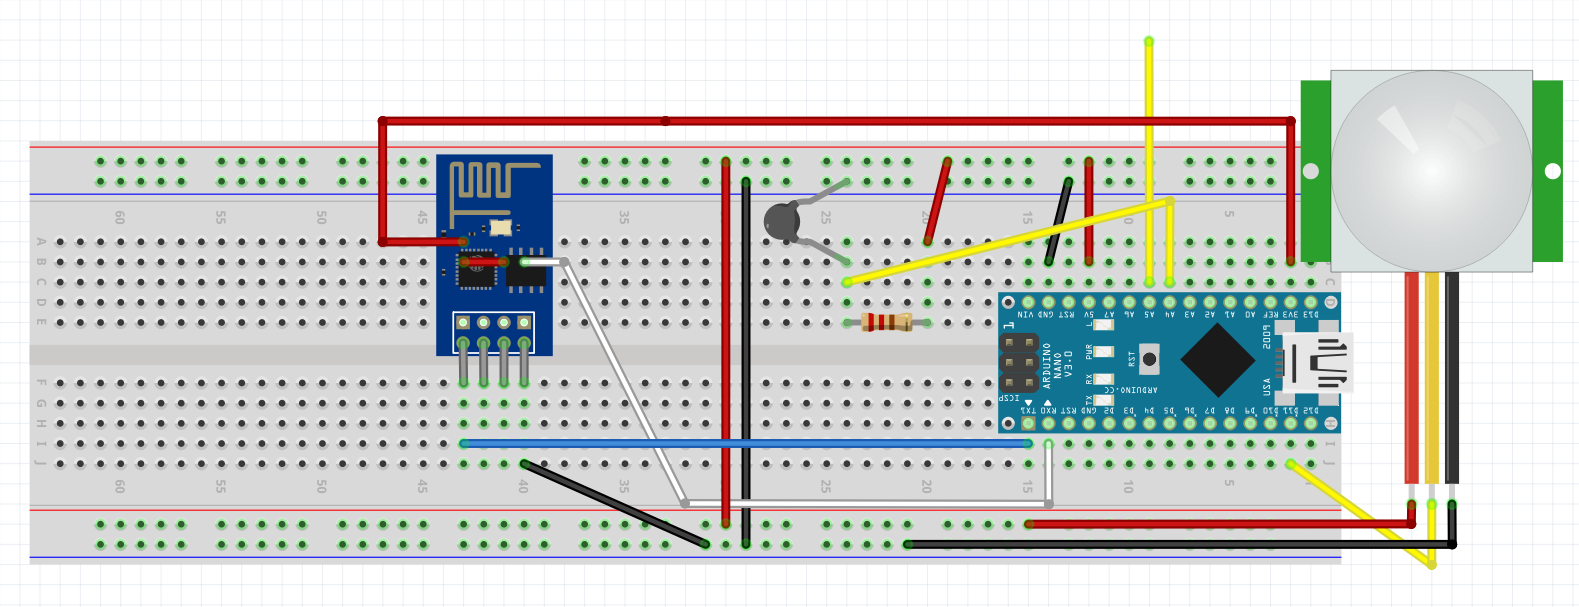
\includegraphics[width=0.6\linewidth]{images/cablage.png}
  \caption{Câblage du microcontrôleur}
  \label{arduino_cablage}
 \end{center}
\end{figure}

\newpage

\section{Software}

D’un point de vue du software, il faut que le microcontrôleur soit capable de lire les informations des différents capteurs mais qu’il puisse aussi générer à partir de cette lecture un type d'information exploitable. Une structure de base de code a été fournie. Elle est axée sur une optimisation de la mémoire, assez réduite, de l’Arduino et elle est complétée par les fonctions nécessaires.\\ 

Le PIR n’envoie que deux signaux : présence ou pas de présence. Quant à la valve thermostatique, il s’agit d’un simple signal analogique. En fonction de celui-ci, on connaîtra aisément son degré d’ouverture compris entre 0 et 100 \%.\\

Pour la mesure de la température, le calcul est un peu plus complexe. D’abord, ce qui sort du senseur est une valeur analogique comprise entre 0 et 1024 et qui représente la tension au borne de la thermistance. Elle dépend bien entendu de la température du milieu. La valeur de 4,64V est utilisée dans la relation de conversion car c'est la tension effective que délivre l’Arduino, et pas 5V. Ceci produit un biais sur la mesure de température si elle n'est pas corrigée.\\

Une fois la tension aux bornes de la thermistance connue, on peut déterminer sa résistance en effectuant un simple calcul de diviseur de tension. C’est en utilisant cette valeur qu'il est possible de déterminer la température de l’environnement grâce à la relation Steinhart-Hart\cite{datash} :

\begin{align}
\label{steinhart}
 T(R) = (A_{1}+B_{1} ln \frac{R}{Ref} + C_{1} ln^{2}\frac{R}{Ref} + D_{1}ln^{3}\frac{R}{Ref})^{-1}
\end{align}

Les constantes de cette relation sont déterminées grâce à la datasheet de la thermistance (voir Table \ref{datasheet_constantes}\cite{datash}). Tous les détails correspondants aux calculs se trouvent dans le code.


\begin{table}[h]
 \begin{center}
  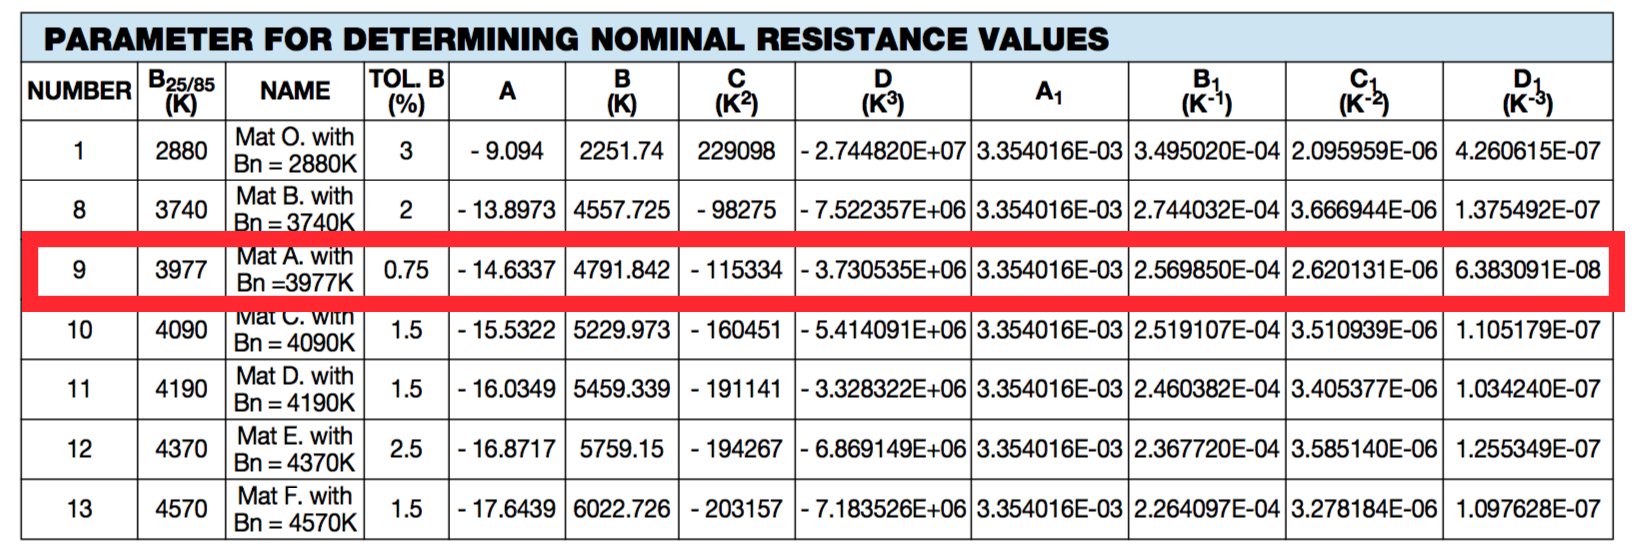
\includegraphics[width=0.6\linewidth]{images/constantes.png}
  \caption{Tableau des constantes utilisées de la datasheet du thermistor}
  \label{datasheet_constantes}
 \end{center}
\end{table}

Les Figures \ref{setup_behav_dia} et \ref{loop_behav_dia} illustrent l'implémentation du microcontrôleur. On y retrouve les deux étapes par lesquelles passent l'Arduino: le \texttt{setup} et le \texttt{loop}.\\ 


\begin{figure}[h]
 \begin{center}
  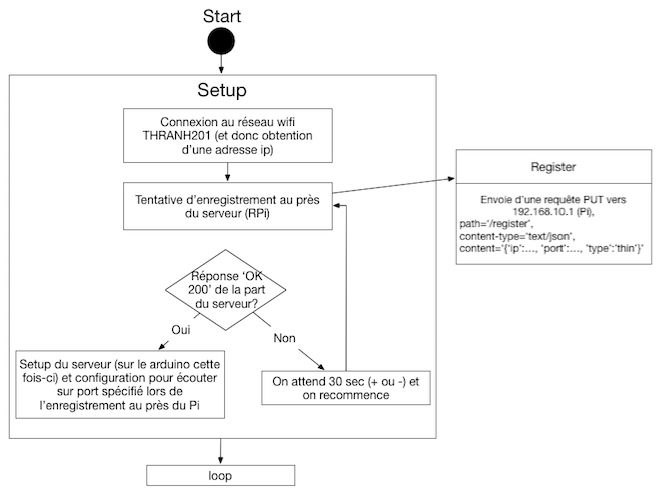
\includegraphics[width=\linewidth]{images/setup_behav_dia.png}
  \caption{Schéma des étapes d'initialisation d'un arduino}
  \label{setup_behav_dia}
 \end{center}
\end{figure}

Le \texttt{setup} se lance à la mise sous tension de l'Arduino et une seule fois. Il est donc logique d'y retrouver la fonction d'initialisation de connexion au Wi-Fi du serveur et celle d'enregistrement.\\

\begin{figure}[h]
 \begin{center}
  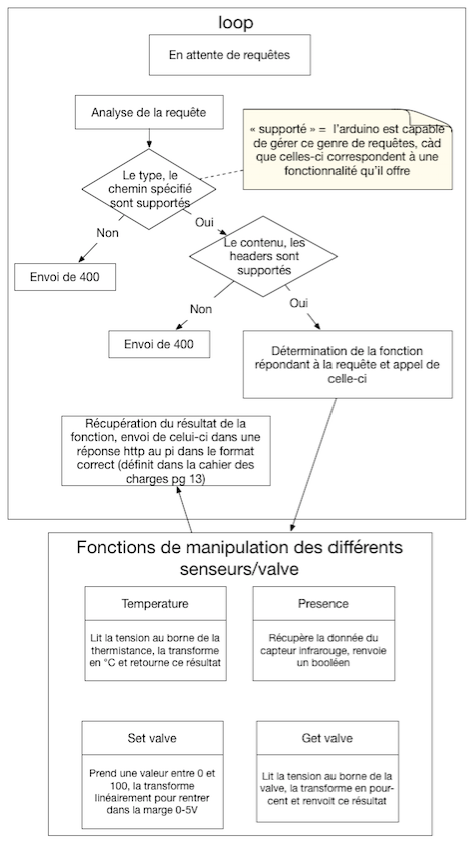
\includegraphics[width=0.7\linewidth]{images/loop_behav_dia.png}
  \caption{Schéma du comportement d'un arduino}
  \label{loop_behav_dia}
 \end{center}
\end{figure}

Le \texttt{loop}, quant à lui, est la boucle qui tourne tant que l'Arduino est sous-tension. Il vérifie à intervalle régulier qu'aucune requête ne lui est adressée. Dans le cas échéant, il découpe la requête et compose sa réponse en fonction de celle-ci. Si elle est bien adressée, alors il renvoie l'information demandée en respectant le protocole HTTP. Sinon, il envoie la réponse \og 400 \fg ~au serveur.\\ 



\newpage
%--------------------------------------------------------------------------------------
%	THERMOSTAT CENTRAL
%--------------------------------------------------------------------------------------

\chapter{Thermostat central}

\section{Serveur}

Cette partie est dédiée à la description du module \texttt{ThermoServer} dont le but principal est de gérer les Arduino connectés (dès la connexion et pendant la récolte des mesures). 

Il a été implémenté de façon à répondre strictement à la description du protocole de communication du cahier des charges. Son fonctionnement global est synthétisé sur la Figure \ref{server_behav_dia}.

\begin{figure}
\centering
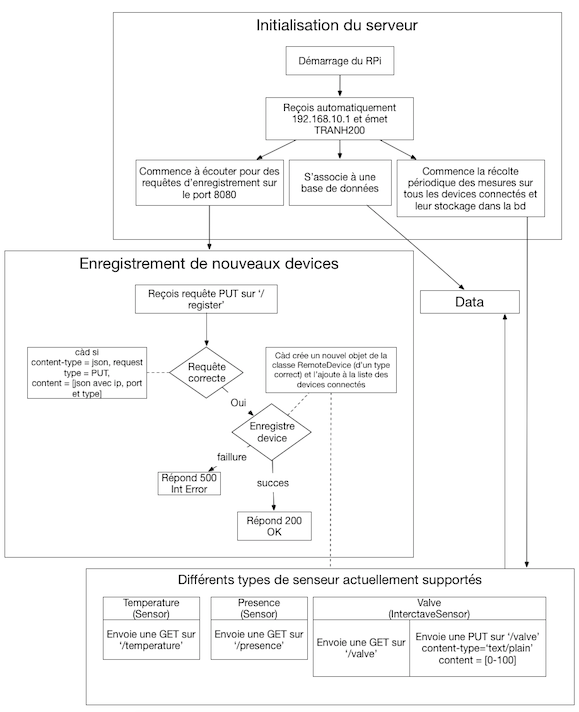
\includegraphics[width=\textwidth]{images/server_behav_dia.png}
\caption{Schéma du comportement du serveur}
\label{server_behav_dia}
\end{figure}


L'implémentation est telle qu'il est très facile de créer et de gérer de nouveaux types de senseur (autres que ceux de type \og thin\fg ~et \og outside\fg  ~demandés dans le cahier des charges).

\subsection{Implémentation}
\begin{figure}
\makebox[\textwidth][c]{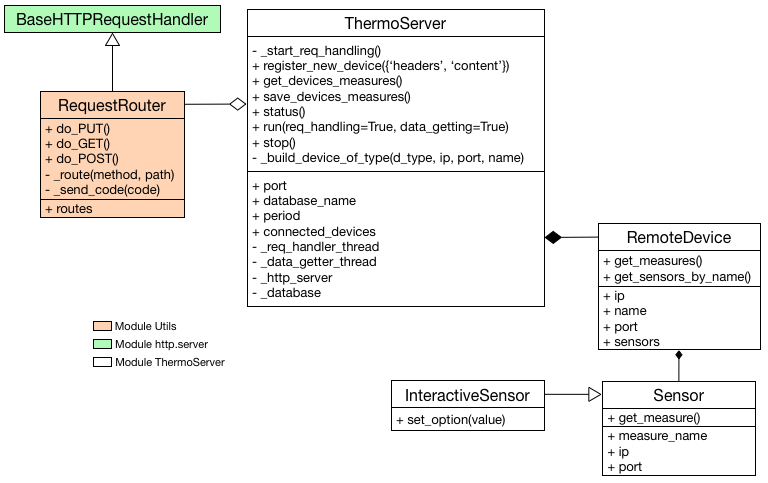
\includegraphics[width=1.15\textwidth]{images/ThermoServer_class_diagram.png}}
\caption{Diagramme de classes du module ThermoServer}
\label{ThermoServer_class_diagram}
\end{figure}
Le protocole de communication s'appuie sur un ensemble de classes qui interagissent entre elles, effectuant chacune une tâche bien précise (décrites brièvement dans le diagramme de classes présenté à la Figure \ref{ThermoServer_class_diagram}\footnote{Les diagrammes de classes présentés dans ce rapport s'inspirent des règles proposés par l'UML mais ne sont pas strictement corrects du point de vue de ce langage. Leur but étant principalement documentaire, une trop grande rigueur n'a pas été jugée utile.}. Chacune d'elles sont détaillées dans les sections suivantes.

\subsubsection{\texttt{ThermoServer}}
\texttt{ThermoServer} est la classe principale de ce serveur. Son but est de s'occuper simultanément de l'enregistrement des Arduino, de la récupération et de l'enregistrement de leurs mesures dans une base de données et, à l'avenir, de la programmation de l'horaire de contrôle des vannes thermostatiques connectées. Ces fonctions sont également réparties sur les autres classes de ce module ainsi que sur les modules \texttt{Data}, \texttt{Utils} et ceux qu'il faudra encore développer et qui géreront l'aspect réactif et l'intelligence du thermostat.\\


Plus techniquement, cette classe est initialisée au démarrage du Raspberry et lance un premier thread consacré au serveur enregistrant les Arduino qui tentent de se connecter (à l'aide de la classe \texttt{RequestRouter} décrite dans la partie \ref{Utils}), et un second récoltant périodiquement les mesures renvoyées par les thermostats auxiliaires connectés et les stockant dans une base de données dédiée. A l'avenir, cette classe enverra les requêtes de contrôle des vannes thermostatiques.


\subsubsection{\texttt{RemoteDevice}}

Cette classe sert d'interface de communication pour les Arduino. Une instance de celle-ci est créée à chaque connexion d'un nouveau Remote Device et permettra d'envoyer chaque requête pour récupérer chacune de ses mesures et pour contrôler ce qui est modulable (les vannes par exemple).

De façon plus technique, cette classe est décrite par une adresse IP et un port permettant la communication avec l'Arduino, par un nom identifiant ces mesures et une liste de senseurs qui sont branchés sur ce thermostat auxiliaires. Cette liste permet de créer tout type de Remote Device, composé de plusieurs senseurs, tels qu'une thermistance, un capteur de présence ou même d'humidité, ou tout autre type de mesures imaginables et compatibles avec le circuit et le code de l'Arduino. 

Grâce à cette implémentation modulaire des Remote Devices, il est possible de créer des objets connectés de tout type et pas seulement de type "thin" ou "outside" comme décrit dans le cahier des charges. L’évolution et l'expansion du projet est rendue beaucoup plus facile sans pour autant compliquer l'implémentation de ce qui est demandé.

%to do : RequestRouter n'est expliqué qu'après. Il faudrait au moins mettre une petite phrase pr dire qu'il sera expliqué plus bas non? Quand j'ai lu le rapport j'ai d'abord cru que t'avais oublié d'en parler 
% Done

\subsubsection{\texttt{Sensor}}
Une instance de cette classe permet simplement de récupérer la mesure du senseur correspondant. Par exemple, si l'on imagine un Arduino sur lequel est connecté une thermistance et configuré pour renvoyer la température ambiante en réponse à une requête de type \texttt{GET} sur le chemin \texttt{\\temperature}, cet objet de type \texttt{Sensor} permettra d'envoyer cette requête et de récupérer la température. \\

Dans le cadre du protocole de communication implémenté ici, un objet de type \texttt{Sensor} est créé pour chaque senseur physique branché et configuré à chaque Remote Device connecté au serveur.

\subsubsection{\texttt{InteractiveSensor}}

Cette classe hérite de la classe \texttt{Sensor} décrite ci-dessus en ajoutant la possibilité d'envoyé une requête de type \texttt{PUT} à un senseur pour le contrôler à distance. Typiquement, cette classe permet de récupérer ET de modifier l'état d'ouverture d'une vanne thermostatique.

%%%%%%%%%%%%%%%%%%%%%%%%%%%%%%%%%%%%%%%%%%%%%%%%%%%%
%  DATA
%%%%%%%%%%%%%%%%%%%%%%%%%%%%%%%%%%%%%%%%%%%%%%%%%%%%

\section{Gestion des données}

\subsection{Introduction}

\paragraph*{}
  Afin d'implémenter une analyse intelligente des habitudes de l'utilisateur, un système de stockage de données est nécessaire. Deux options sont envisageables. Soit une structure sous forme de fichier, soit une autre utilisant les bases de données. Des recherches ont été menées pour déterminer quel système serait le plus adéquat. Il en est ressorti que les bases de données correspondent mieux à la problématique. En effet, celles-ci sont plus rapides, plus simples à manipuler et s'adaptent facilement à différentes tailles de jeux de données. De plus, en Python, de nombreuses bibliothèques les concernant existent, et certains types de bases de données, comme par exemple SQLite, y sont intégrés par défaut. Les raisons citées précédemment ont dès lors mené à une décision en faveur des bases de données.
  
\subsection{Choix de la base de données}
\paragraph*{}
  Il existe différentes bases de données, chacune ayant ses avantages et inconvénients. Une analyse comparative des plus populaires a été réalisée et SQLite a été choisi. La Table \ref{tableau db} justifie cette décision. 

\begin{table}[h]
   \centering
   \begin{tabularx}{\linewidth}{|c||X|X|X|}
      \hline
       Caractéristiques & \centering{SQLite} & \centering MySQL & \centering PostgreSQL \tabularnewline
      \hline
      Installation & SQLite est déjà implémenté dans Python.\cite{table1} & Installation d'un serveur MySQL nécessaire.\cite{table2} & Installation de PostgreSQL nécessaire.\cite{table3}\tabularnewline
      \hline
      Types de données supportés & NULL, INTEGER, REAL, TEXT, BLOB.\cite{table4} & Complet, accepte également des entrées de type \og Date \fg.\cite{table5} & Complet, accepte également des entrées de type \og Date \fg.\cite{table6} \tabularnewline
      \hline
    Stockage de la base de donnée & La base de donnée est condensée en un seul \og fichier \fg ~stocké directement dans la mémoire (Du Raspberry dans ce cas).\cite{table7}  & La base de donnée est stockée sur un serveur au quel doivent se connecter les utilisateurs.\cite{table8}& La base de donnée est stockée sur un serveur au quel doivent se connecter les utilisateurs.\cite{table9}\\    
		\hline
	\end{tabularx}
\caption{\label{tableau db} Tableau comparatif des différentes bases de données étudiées}
\end{table}

\subsection{Implémentation}

\begin{figure}
\centering
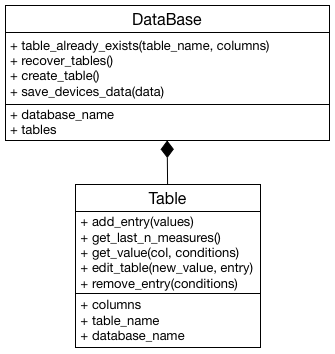
\includegraphics[width=0.5\textwidth]{images/Data_class_diagram.png}
\caption{Diagramme de classe du module \texttt{Data}}
\label{Data_class_diagram}
\end{figure}

\paragraph*{}
L'implémentation actuelle du module \texttt{Data} consiste en deux classes, \texttt{Database} et \texttt{Table}, s'occupant des interactions entre une base de données et le serveur pour la première, et entre une table et le serveur pour la seconde. La structure adoptée pour l'instant crée une base de données et, à chaque fois qu'un Remote Device se connecte au serveur, une table portant son nom est générée comme le montre la Figure \ref{current_structure}. Le détail des classes est schématisé à la Figure \ref{Data_class_diagram} et développé dans les paragraphes suivants.
   
\begin{figure}
\centering
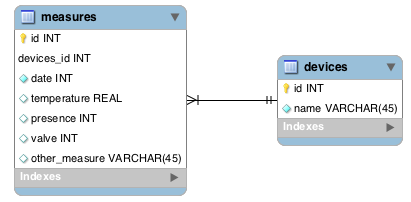
\includegraphics[width=0.75\textwidth]{images/better_structure.png}
\caption{Schéma de la structure plus adaptée envisagée}
\label{Better_structure}
\end{figure}

\begin{figure}
\centering
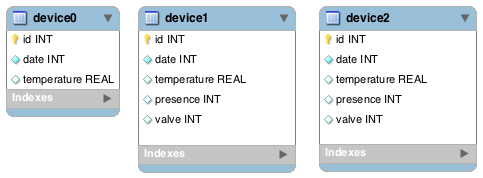
\includegraphics[width=0.9\textwidth]{images/current_structure.png}
\caption{Schéma de la structure présentement implémentée de la base de donnée}
\label{current_structure}
\end{figure}

\subsubsection{Classe \texttt{Database} }
\paragraph*{}
   La classe \texttt{Database} est l'intermédiaire entre le serveur et la base de données. Elle permet, entre autres, de créer une base de données, de s'y connecter et d'y créer des tables. Elle a été conçue de telle sorte à ne pas créer d'instabilité. En effet si le serveur vient à redémarrer, une instance identique à celle en cours précédemment est créée afin que le code continue à s'exécuter de la manière souhaitée.
    
\subsubsection{Classe \texttt{Table}}
\paragraph*{}
	Quant à elle, la classe \texttt{Table} permet d'effectuer des manipulations sur une table, comme par exemple ajouter des entrées ou en supprimer. Elle a principalement été conçue en généralisant la syntaxe du module \texttt{sqlite3} de façon à créer des méthodes d'un plus haut niveau d'abstraction et élégantes d'utilisation.
    
\subsection{Regard critique sur l'implémentation de la base de données}
\paragraph*{}
	L'implémentation actuelle du module \texttt{Data} n'est pas optimale. Cette manière de faire a été décidée tôt dans la conception du serveur. Elle a mené à de longues discussions et semblait être une bonne solution dans la mesure où elle correspondait à la structure globale du code qui consiste une indépendance des différents Remote Devices afin de rendre ce dernier plus flexible. Par la suite, il s'est avéré que ce n'est pas une bonne structure à adopter. En effet, ce n'est pas une façon propre de faire car cela va à l'encontre des règles de bonnes pratiques. Lorsqu'une base de données est utilisée, afin d'optimiser les performances, une seule et unique table est utilisée. De plus, si il y a des problèmes de connexion et que le serveur oublie l'existence des Remote Devices, à chaque fois que ceux-ci se reconnecteront des nouvelles tables seront créées, potentiellement en très grands nombres.
    
\paragraph*{}
	Ces raisons motivent le fait qu'une nouvelle structure soit implémentée dès que possible. Celle-ci s'articule comme l'indique la figure \ref{Better_structure}. Une seule grande table contiendra toutes les données de tous les Remote Device, peu importe leur type, et aura en plus un identifiant qui fera le lien avec le Remote Device d'où proviennent les données correspondantes grâce à une table de jointure. De cette manière, le système gagne en flexibilité car il est possible d'ajouter n'importe quel type de capteur\footnote{Dans une perspective de développement ultérieur du projet, par exemple ajouter des capteurs d'humidité,...} sur les Remote Devices, ce qui est le résultat recherché.
    
    %to do: j'aurai mis les graphiques ici vu que c'est dans ce paragraphe que tu y fais référence

\section{Module \texttt{Utils}}
\label{Utils}
Ce module ne contient (pour le moment) que deux classes : \texttt{RepeatingTimer} et \texttt{RequestRouter}. \\

Il a pour but de contenir des classes ou plus généralement des outils qui sont complètement indépendants du projet (mais utiles à celui-ci) et qui pourraient donc être facilement utilisables pour un quelconque autre projet. Outre le fait que la séparation des classes génériques leur permet d'être réutilisées dans d'autre projet, se pliant ainsi aux règles de bonnes pratiques, la construction d'un module séparé contenant ces classes permet d'alléger les autres modules et de les rendre plus compréhensible.\\


Ces deux classes sont donc construites de façon générique et accomplissent des taches élémentaires.


\subsection{RepeatingTimer}
\begin{figure}
\centering
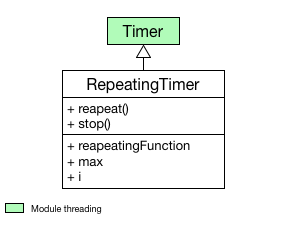
\includegraphics[width=0.5\textwidth]{images/RepeatingTimer_class_diagram.png}
\caption{Diagramme de classe pour RepeatingTimer}
\end{figure}

La seule fonction de cette classe (héritant de la classe \texttt{Timer} du module \texttt{threading} de python) est d'appeler une fonction spécifiée à intervalle régulier. \\

Elle est utile, dans ce projet, à la collecte des mesures régulière du serveur sur les remote devices connectés. \\

\subsection{RequestRouter}
\begin{figure}
\centering
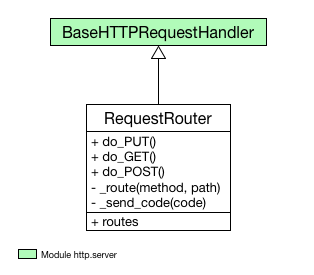
\includegraphics[width=0.5\textwidth]{images/RequestRouter_class_diagram.png}
\caption{Diagramme de classe pour RequestRouter}
\end{figure}

Cette classe, héritant de \texttt{BaseHTTPRequestHandler} fournie dans le module \texttt{http.server} de python 3, a pour but d'écouter sur un port spécifié pour d'éventuelles requêtes et de les "router" vers un callback spécifié en fonction de la méthode http et du chemin de la requête.\\

Elle est totalement générique puisque n'importe quelle requête peut déclencher n'importe quelle fonction (pour peu qu'elle soit configurée correctement) et peut-être utilisée dans n'importe quel cas nécessitant un serveur.\\

Dans le cadre spécifique de ce projet, cette classe est utile à la réception et au traitement des requêtes d'enregistrement des remote devices.



\section{Debugage}

Un système de logging est implémenté dans tous les modules pour garder une trace de chaque éventuelle erreur, disfonctionnement, anomalie lors du fonctionnement du serveur. Le dépannage sera alors simplifié lors d'une utilisation réelle et le debugage est plus rapide lors du développement dès lors que l'origine des erreurs est plus facilement identifiable. Il est ainsi possible dès le lancement du serveur d'indiquer quels types (niveau de gravité) de messages doivent être affichés et/ou stockés dans un fichier journal.


%\newpage
%--------------------------------------------------------------------------------------
%	TESTS
%--------------------------------------------------------------------------------------

%\chapter{Tests}

%Des tests ont été réalisés afin de terminer la validité de toutes les implémentations. Tant celles des périphériques de l’Arduino que du Raspberry pi. Ces tests permettent de vérifier que le dispositif fonctionne normalement dans un maximum de conditions différentes. Le tout dans le but d’améliorer le thermostat et de vérifier son bon fonctionnement dans différentes utilisations. Le principe du test est d’effectuer une dizaine de fois la même opération et de vérifié que le résultat obtenu est bien celui attendu.\\

%\section{Tests sur les \og remotes devices \fg}

%Comme mentionné précédemment, les \og remotes devices \fg sont composés de plusieurs capteurs différents. Les différents tests à réaliser concerneront : Le capteur de présence, le thermistance, le module wifi, et la réunion de ces trois modules.\\

%\subsection{Validation du capteur de présence}

%Ce capteur de présence sera testé à l’aide du code fourni en annexe ??. Il a été placé dans une pièce initialement vide et différentes personnes sont rentrées et sorties. Des déplacements à courte distance ont également été effectué afin d'échantillonner la distance d'utilisation. La distance est finalement apparue comme sans effet sur les tests.\\ 

%\subsection{Validation du modèle de la thermistance} 

%Ce thermistance a été testé dans diverses conditions, tant intérieures qu’extérieures afin d’obtenir une vaste plage de températures dans lequel sa validité pourrait  confirmée à l'aide d'un autre thermomètre. Ces tests informels ont donc confirmés le fonctionnement de cet fonction du remote device.\\

%to do: les 2 références aux annexes à remplir, le tableau de donnée à remplir??

%RETODO :  Je n'ai pas réussi a faire fonctionner le raspberry et l'arduino chez moi,
%RETODO : Je pensais que ces codes sera placés en annexes ? Ce n'est pas le cas ?
%RERETODO : Pas de code dans le rapport, espèce d'insouciant!! :p (Steph), au pire on peut les mettre dans les délivrable dans un dossier test. 
%RERETODO: (soufiane) Alors on supprime les tableaux?? Je viens de voir que les tests ont pas été fait et demain je suis pas chez moi avant tard le soir....on m'a pas dit qu'il fallait que je fasse les tests c'est dommage
%\section{Tests sur le thermostat central}

%\subsection{Validation du serveur}
%to do: y a rien pour ca? Meme pas dire qu'on va le faire au deuxième quadri?
%RETODO : Done

%Des tests informels ont été réalisés afin de tester le fonctionnement du serveur. Le remplissage de la base de données implique que le serveur est opérationnel mais une méthode de test plus rigoureuse envisageant un maximum de cas possible sera rédigée et effectuée lors du deuxième quadrimestre.\\

%\subsection{Validation de la base de donnée}

%La base de donnée doit être soumis à de nombreux cas de figures afin de déterminer sa validité. Le premier test est de lancer le serveur sur le raspberry avec la base de donnée connectée à un Arduino et de lui demander de stocker les données récoltées par le Raspberry. Ce test fut effectué avec succès, ce qui confirme que la méthode \og add\_entry \fg et \og create\_table \fg fonctionne.\\

%Une autre méthode à tester est  \og table\_already\_exists \fg et \og recover\_table \fg. Ce test consiste à débrancher le Raspberry durant son fonctionnement afin de simuler une coupure de courant et de le relancer par après afin de voir si les données qu'il collectera à nouveau sur le même Arduino seront insérées dans la même table oui ou non. Ce test fut concluant également.\\

%\section{Tests à effectuer à posteriori}

%Tous ces tests permettent d'attester du fonctionnement effectif de la base de donnée, du serveur, de l'arduino, du capteur de présence, etc. Mais ils ne constituent pas en réalité d'un protocole de test en bonne et due forme. Une méthode de test bien plus rigoureuse, consistant. De plus, des modules tels que la base de donnée prendront une forme nouvelle, il sera donc nécéssaire d'adapter les tests réalisés à la nouvelle structure.\\



%to do: repréciser que puisqu'on va le changer au deuxième quadri et que donc on va faire des tests spécifiques aux nouvelles bases de données non? Faudrait aussi parler que nos tests seront plus rigoureux aux deuxième quadri pour l'ensemble des modules et que ca c'est juste des tests pour voir si ca marche

%RETODO : done

\newpage
%----------------------------------------------------------------------------------------
%	FONCTIONNEMENT DE GROUPE
%----------------------------------------------------------------------------------------

\chapter{Fonctionnement de groupe}

	Afin d’atteindre les objectifs du projet le plus rapidement et le plus efficacement possible, il était important d’établir une bonne organisation du travail en groupe afin de maximiser la productivité du groupe et de répartir la quantité de tâches à effectuer par chacun de manière équitable. Quelques outils ont donc été mis en place dès la première semaine dans cette optique.\\

	Pour commencer, le plus important était de définir comment les informations transiteraient. Un groupe privé sur Facebook a été choisi pour la communication informelle en dehors des réunions, l’avantage étant de pouvoir conserver un historique de ces conversations. Le transfert des documents, codes, parties de rapport,... s’effectue quant à lui via une Dropbox qui permet d'archiver et de partager tous ces fichiers de façon simple et efficace. Il a également été décidé que le rapport serait rédigé en \LaTeX sur \og Overleaf\footnote{\url{https://www.overleaf.com/}} \fg, cette plate-forme permettant la modification en temps réel du document par tous les membres de l’équipe.\\

	La fréquence des réunions fut fixée au rythme de deux par semaines. Une avec le tuteur du projet afin de le tenir au courant des avancées réalisées lors de l’autre réunion qui concerne uniquement les membres du groupe. Lors de ces rencontres hebdomadaires, chacun se doit de comprendre les avancée exposées par les autres membres du groupe afin d’obtenir des connaissances homogènes dans tous les domaines. Cette fréquence permet de ne pas oublier de travailler chaque semaine sur le projet. Il arrive que des réunions supplémentaires soient organisées en équipe lorsque le besoin s’en fait sentir ou qu’une deadline approche.\\

	Ces réunions se tiennent, sauf cas de force majeure, à la Bibliothèque des Sciences et Techniques de l’ULB, principalement pour des raisons de proximité. Durant ces réunions, un membre est désigné et joue le rôle de secrétaire et d’animateur. La fusion de ces deux rôles a été décidée en raison de la taille du groupe. La tâche de de cette personne est d’envoyer l’ordre du jour aux autres membres au moins 24 heures avant la réunion, de l’animer ensuite et d’en rédiger le procès-verbal par après. Ce poste est attribué à une autre personne toutes les deux semaines sur base volontaire afin de ne surcharger personne de travail.\\
    
\newpage

%--------------------------------------------------------------------------------------
%	PERSPECTIVES D'EVOLUTION
%--------------------------------------------------------------------------------------

\chapter{Perspectives d'évolution}

En ce qui concerne de la suite du projet, il a été décidé de maintenir la même méthode de travail,à savoir en planifiant les tâches en se basant sur le cahier des charges. Le premier quadrimestre a été essentiellement consacré à la familiarisation avec les différents outils. Raspberry Pi, programmation orientée objet, Arduino, base de données étant autant de concept qu'il a fallu apprendre à utiliser et maîtriser. C'est pourquoi les milestones une et deux ont été abordé jusqu'à présent. \\

Suivant cette logique, c'est donc bien le développement des milestones trois et quatre qui sera d'actualité au second quadrimestre (voir Figure \ref{planning}), bien que celui-ci soit beaucoup plus court. Il y aura une réflexion qui précédera la mise en place d'un algorithme intelligent suivant les exigences du cahier de charges. Ce planning est potentiellement sujet à des modifications ultérieures mais il reste une bonne base de travail. Il est volontairement "sur-estimé", notamment en ce qui concerne la finalisation du rapport final. Ceci a pour but de pallier aux imprévus comme ceux rencontrés au premier quadrimestre.\\ 



\newpage
\begin{figure}[h]


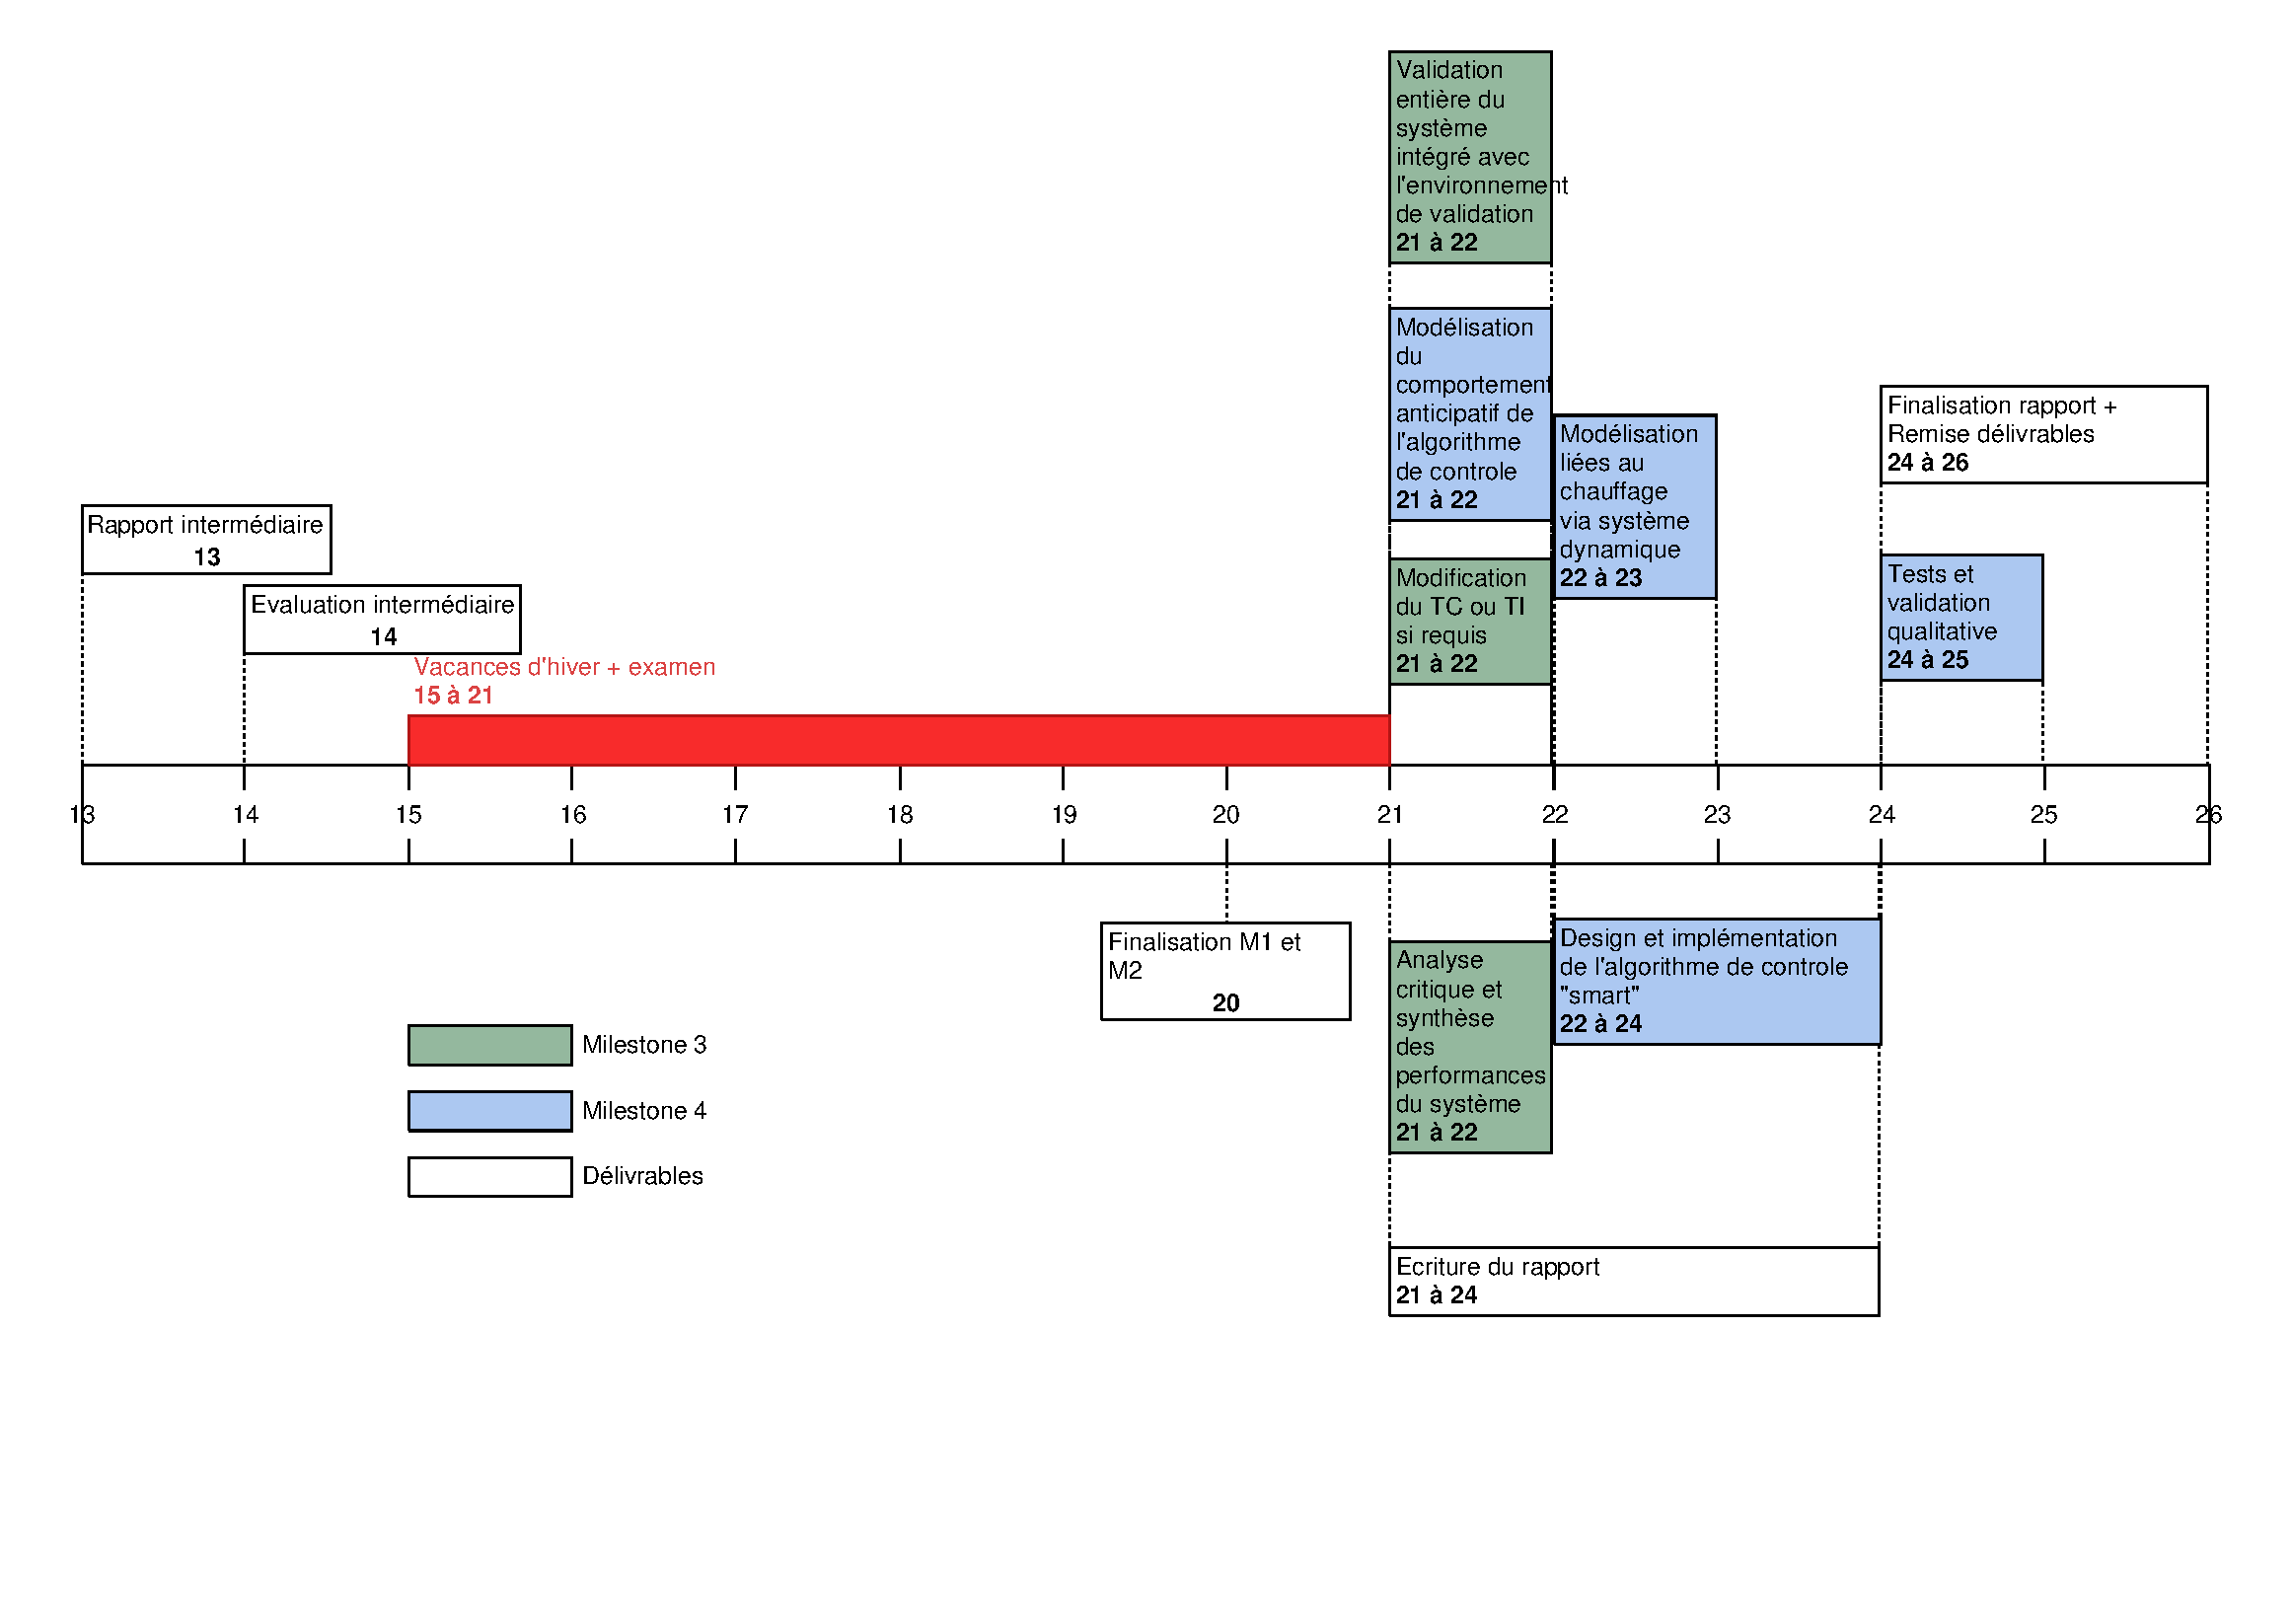
\includepdf[page=1]{pdf/frise.pdf}
\caption{Planning du second quadrimestre}
\label{planning}


\end{figure}

\newpage
%--------------------------------------------------------------------------------------
%	CONCLUSIONS
%--------------------------------------------------------------------------------------

\chapter{Conclusion}

La conception et la visualisation des demandes du projet était la première étape clé du processus de fabrication du thermostat intelligent. L'utilisation du diagramme présenté en Annexe \ref{dia_complet} était le moyen le plus efficace de se représenter l'objectif final. La réalisation du câblage des différents composants a été assez rapidement effectué, tout comme l'implémentation de l'Arduino, bien que parfois celle-ci ait été retardée suite à un manque de matériel.\\

L'autre partie abordée en parallèle concernait le Raspberry. La création d'un serveur était nécessaire, l'implémentation de celui-ci est telle qu'il permet une plus grande flexibilité que celle exigée par le cahier des charges. En effet, on peut y connecter n'importe quel type de Remote Device. Comme exigé dans le cahier des charges, les communications respectent le protocole HTTP.\\

Un stockage des données était nécessaire afin d'implémenter l'analyse intelligente. Une étude a été menée afin de choisir entre les différentes façon de faire et SQLite a finalement été retenu pour sa légèreté, sa simplicité et sa présence par défaut dans Python. L'implémentation actuelle ne respecte pas les conventions et sera prochainement revue. Elle avait été structurée de cette manière car elle semblait plus souple.\\

Le fonctionnement du groupe tel qu'il est à présent semble ne souffrir d'aucun problème en particulier. Il sera donc conservé sauf imprévu lors du deuxième quadrimestre.\\

Le travail restant à fournir est assez conséquent, les milestones une et deux sont presque achevées et les milestones trois et quatre devront être entamées dès le début du second quadrimestre afin de respecter les deadlines. Celui-ci sera entamé par la finalisation des algorithmes de contrôle réactifs. Une fois cette étape achevée, le code intelligent sera implémenté.

%to do: A FAIRE
%RETODO : Almoste done

\newpage

%--------------------------------------------------------------------------------------
%	MEMBRES DU GROUPE
%--------------------------------------------------------------------------------------

\chapter{Membres du groupe}

\begin{minipage}{0.45\textwidth}
\begin{flushleft} 
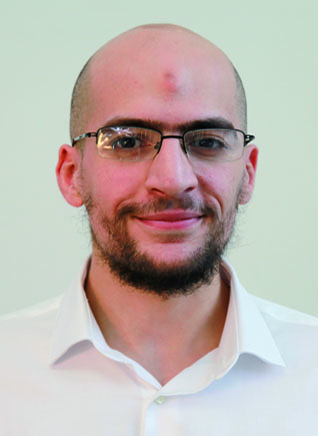
\includegraphics[height=4cm] {photos_membres/Soufiane.jpg}\\
\textsc{Amzur} Soufiane\\
\textsc{000328725}\\
\textsc{soufiane.amz@gmail.com}\\
\end{flushleft}
\end{minipage}
~
\begin{minipage}{0.45\textwidth}
\begin{flushright}
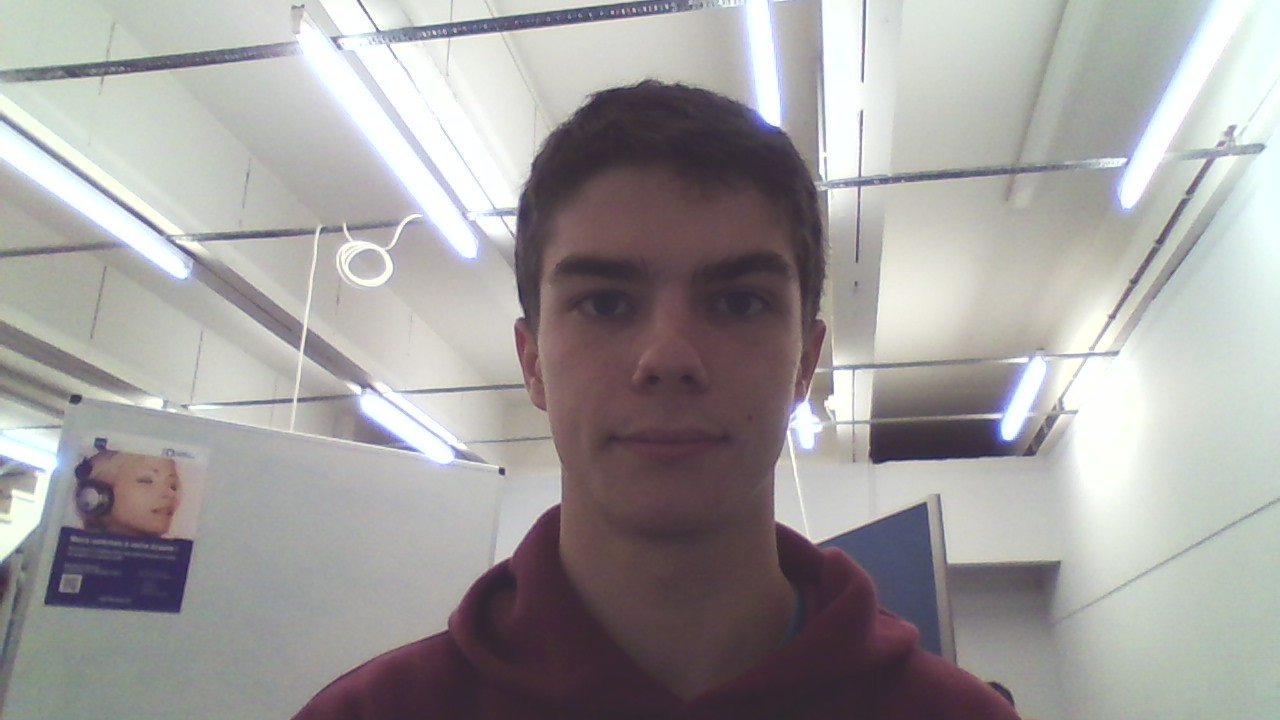
\includegraphics[height=4cm]{photos_membres/Wilson.jpg}\\
\textsc{Daubry} Wilson\\
\textsc{000408780}\\
\textsc{daubry.wilson@gmail.com}\\
\end{flushright}
\end{minipage}

\emph{} \\
\emph{} \\
\emph{} \\
\emph{} \\
\emph{} \\

\begin{minipage}{0.45\textwidth}
\begin{flushleft} 
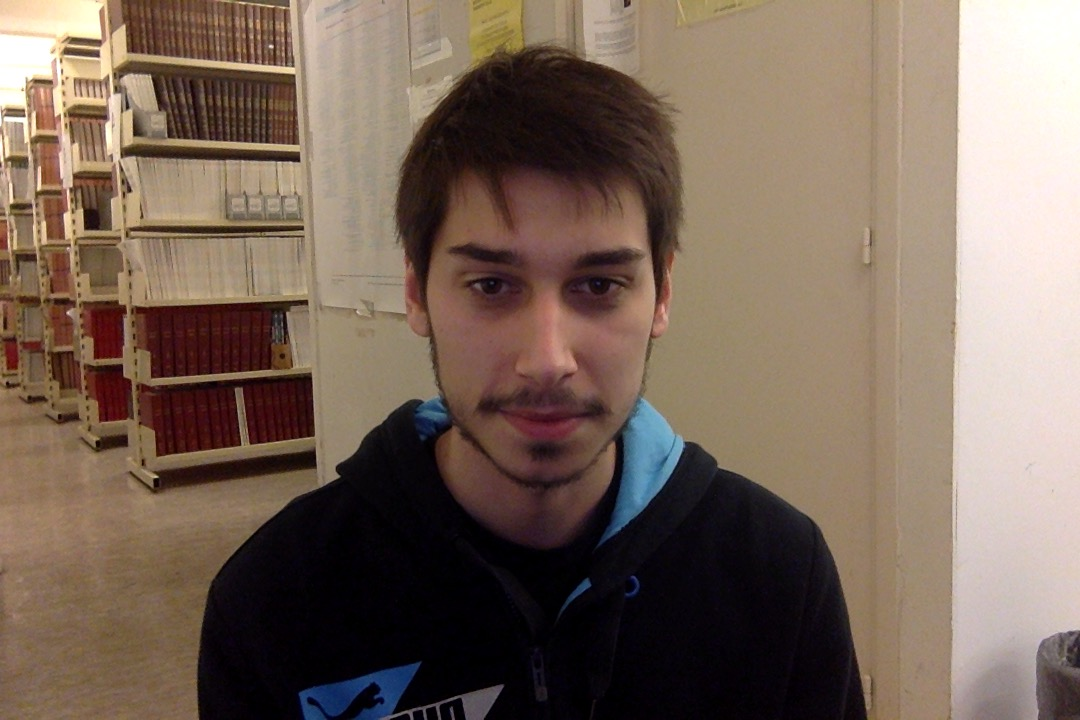
\includegraphics[height=4cm] {photos_membres/Stephane.jpg}\\
\textsc{Sercu} Stephane\\
\textsc{000408643}\\
\textsc{ssercu@ulb.ac.be}\\
\end{flushleft}
\end{minipage}
~
\begin{minipage}{0.45\textwidth}
\begin{flushright}
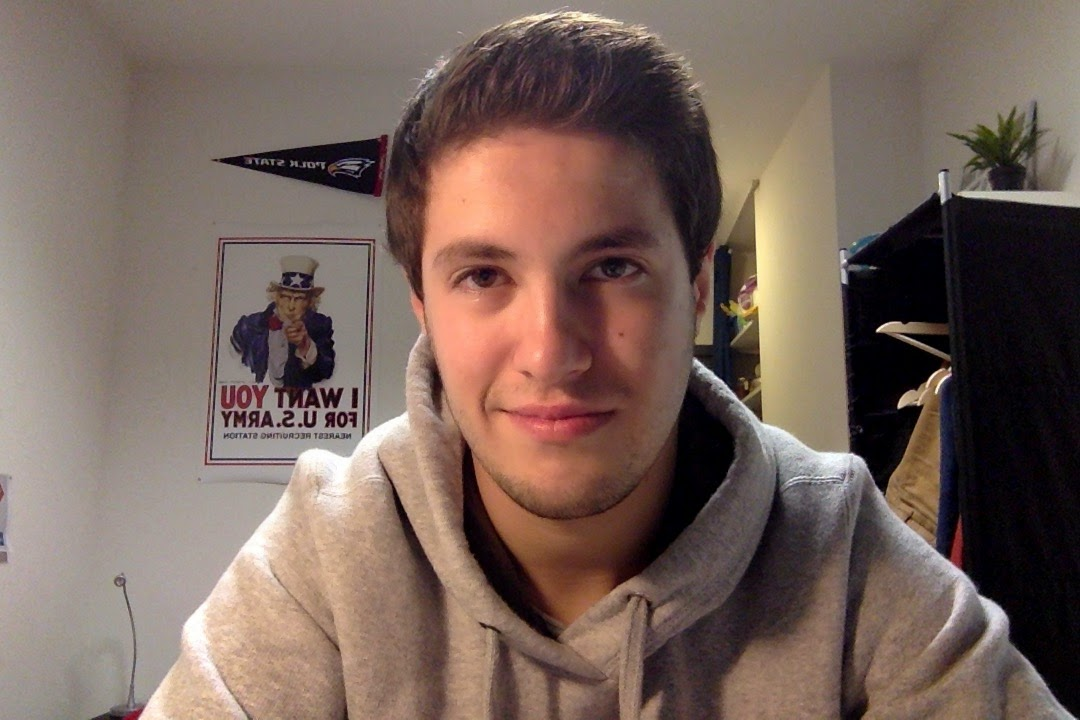
\includegraphics[height=4cm]{photos_membres/Denis.jpg}\\
\textsc{Verstraeten} Denis\\
\textsc{000401967}\\
\textsc{denverst@ulb.ac.be}\\
\end{flushright}
\end{minipage}

\newpage

%to do: ma photo doit etre au mm format que la votre

%RETODO : Prendre nos 4 photos avec le mac de Denis Mais est ce vraiment un probleme ? Ma photo non plus n'a pas les meme dimension

%RERETODO: ok on s'en fout alors lol

\appendix

%======================================================================================
%	ANNEXES
%======================================================================================


%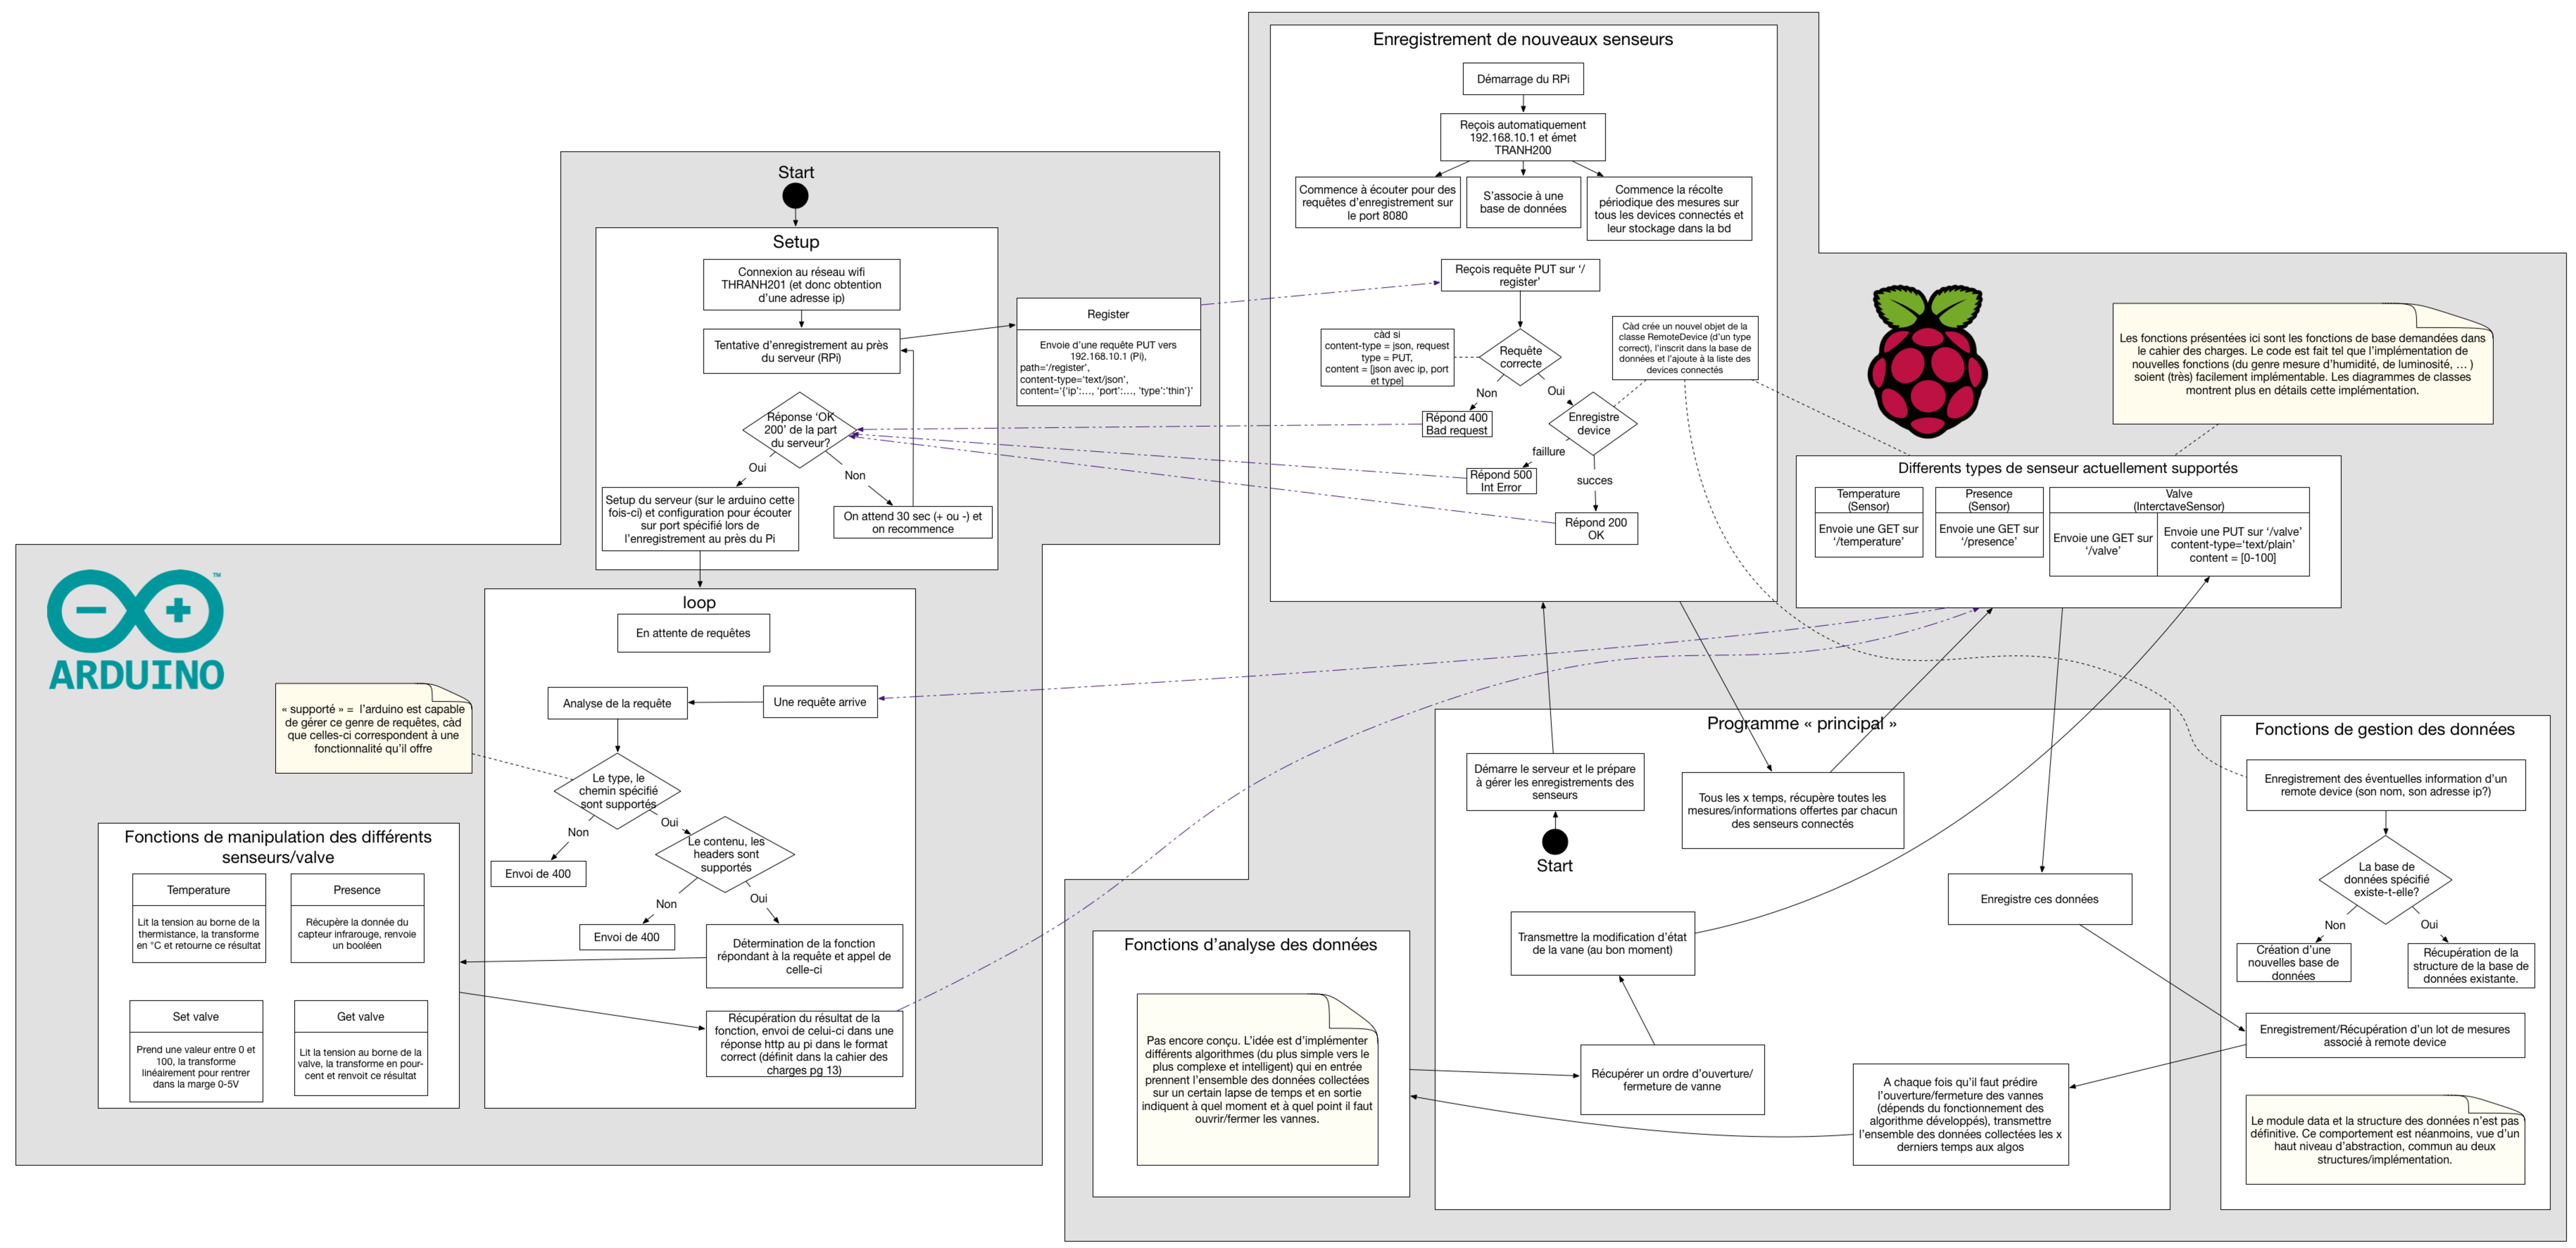
\includepdf[pages={1}, landscape=true, pagecommand=\chapter{Diagramme de comportement global}]{pdf/diagrams_complet.pdf}


\chapter{Diagramme de comportement global}
\label{dia_complet}
Comme expliqué dans la partie Conception, ce diagramme a été créé principalement pour faciliter le travail de groupe. Il offre une vue très synthétique du comportement de l'ensemble du système ainsi que de la façon dont les différentes parties communiquent et interagissent.\\
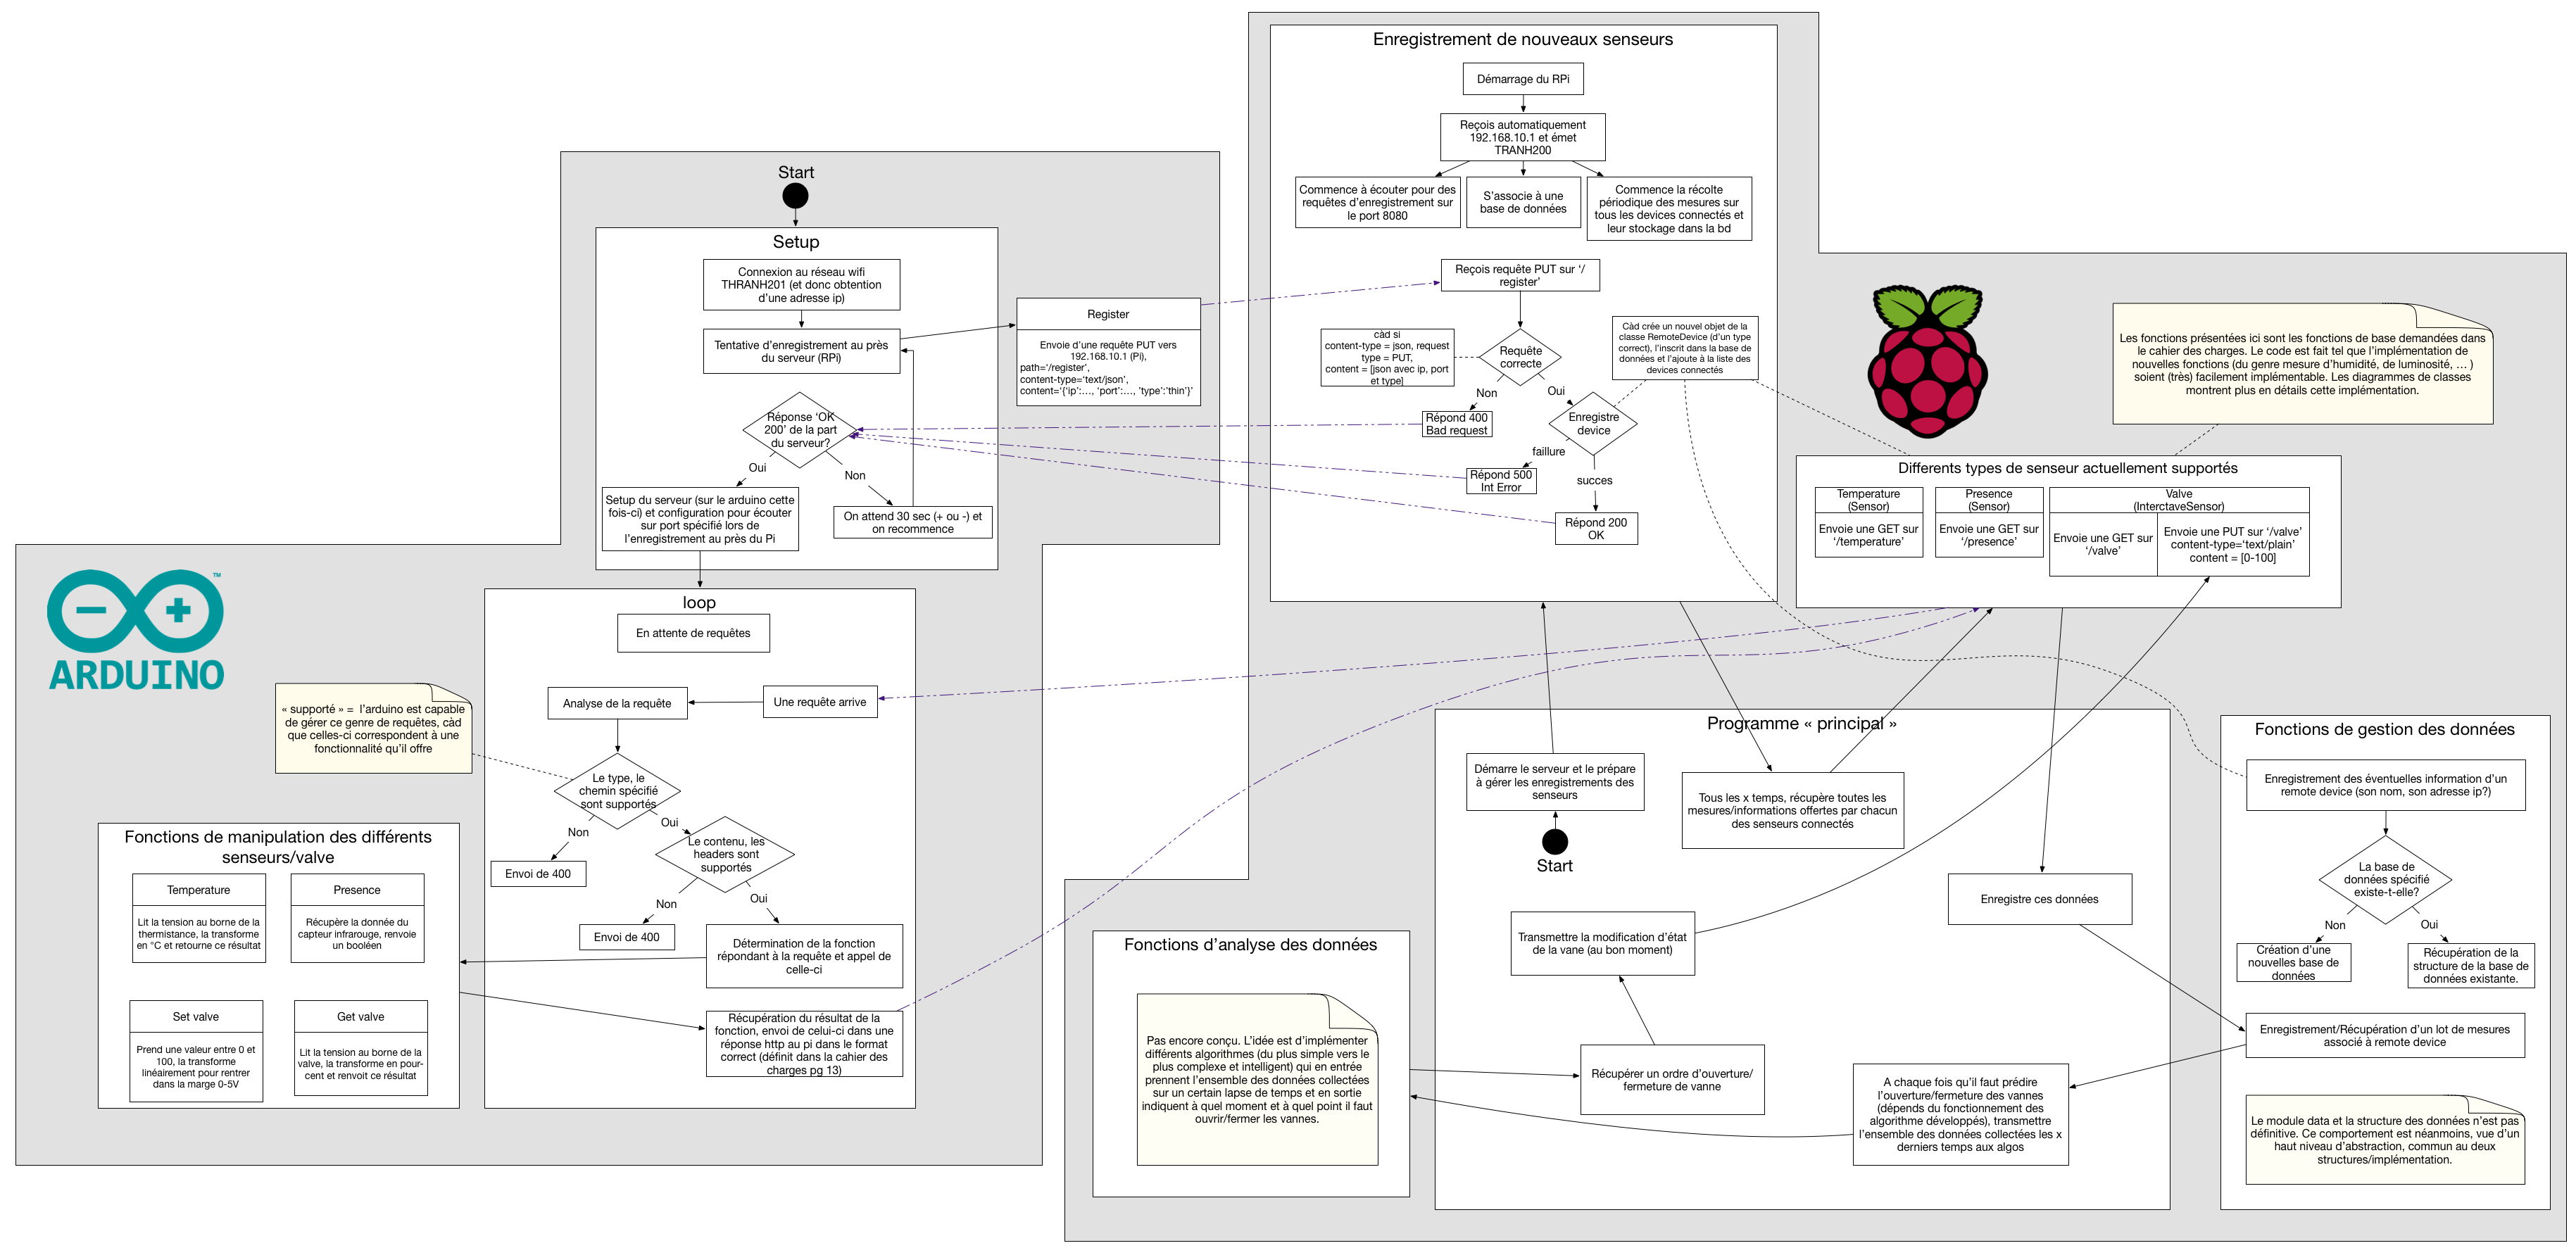
\includegraphics[width=\textwidth]{images/diagrams_complet.png}


% to do : pourquoi 2 fois "chapter"? Regler la lisibilité du schéma qui déborde sur le titre


%--------------------------------------------------------------------------------------
%	CONVENTION DE PROGRAMMATION
%--------------------------------------------------------------------------------------

\chapter{Conventions de programmation}


Dans le but de garder un code propre et maintenable par tous les participants du projet sur le long terme, des conventions et règles de bonne pratique ont été choisies pour être respectées.\\


\section{Code Python}
\begin{itemize}
\item les conventions proposées dans le cours de Thierry Massart \cite{massart}. Notamment pour les docstring, le nommage des classes, des fonctions et des variables,
\item la langue choisie pour le code est l'anglais, pour la simple et bonne raison que c'est la langue universelle des développeurs. Le code n'en est que plus cohérent par rapport aux fonctions prédéfinies.
\item L'orienté objet a été un choix facile : le code n'en est que plus compréhensible, structuré, modulaire et évolutif. 
\item Une attention particulière a été portée à la documentation de chaque méthode/fonction/classe pour éviter une perte de temps à la compréhension et l'analyse du code par les autres membres du groupe et/où par l'auteur lui même dans l'avenir. De cette façon, l'utilisation de ces fonctions est simplifié et ne nécessite que la lecture de la documentation associée pour savoir de quelle façon il faut les appeler et quel type de paramètre il faut leur passer.
\item Les deux modules principaux (\texttt{ThermoServer} et \texttt{Data}) sont accompagnés de diagrammes de classe permettant leur documentation. Ils offrent une vue globale, simplifiée et résumée de leur structure. Cette pratique sera maintenue pour les prochains modules principalement pour son pouvoir documentaire.
\end{itemize}

\section{Code Arduino}

Cette partie a été programmée directement dans le code de base fournis, le style de programmation a donc été calqué sur celui-ci.

%to do : changer les commentaires du code Arduino pour les mettre en anglais..


\newpage

% Il ne faut pas toucher/supprimer ca MERCI :p
% TROP TARD
% CA VA EXPLOSEEEEEEEEER !!!!!
\nocite{int1}
\nocite{int2}
\nocite{int4}
\nocite{int5}
\nocite{int6}
\nocite{int7}
\nocite{int8}
\nocite{ar1}
\nocite{ar2}
\nocite{ar3}
\nocite{ar4}
\nocite{wil1}
\nocite{wil2}
\nocite{wil3}
\nocite{wil4}
\nocite{wil5}
\nocite{s1}
\nocite{s2}

\bibliography{bibliographie/biblio}
\bibliographystyle{plain} 


\end{document}

